\documentclass[11pt]{article}

\usepackage[letterpaper]{geometry}    % set page margins
\usepackage{graphicx}                 % for including images
\usepackage{fancyhdr}                 % customize headers and footers
\usepackage{titlesec}                 % customize section headings
\usepackage{multicol}                 % for multi-column layout
\usepackage{hyperref}                 % for hyperlinks
\usepackage{setspace}                 % for setting the line spacing in footnotes
\usepackage[hang]{footmisc}           % for footnote customization
\usepackage{balance}                  % for balancing columns
\usepackage[numbers]{natbib}          % for bibliography
\usepackage{caption}                  % for figure captions

% Define page margins
\geometry{
    top=0.5in,
    bottom=0.5in,
    left=0.5in,
    right=0.5in,
    headheight=0pt,
    includeheadfoot
}

% Define link colors
\hypersetup{
    colorlinks=true,
    linkcolor=blue,
    filecolor=magenta,
    urlcolor=blue,
    citecolor=blue
}

% Customize header and footer
\pagestyle{fancy}
\fancyhf{}                         % clear default header and footer
\renewcommand{\headrulewidth}{0pt} % remove header rule
\fancyfoot[R]{\thepage}            % page number centered in footer

% Customize section headings
\titleformat{\section}{\normalfont\large\bfseries}{\thesection}{1em}{}
\titlespacing{\section}{0pt}{\parskip}{-\parskip}

% Customize footnotes
\renewcommand{\footnotelayout}{\raggedright\setstretch{1.25}\parindent 0em}
\renewcommand{\footnoterule}{%
    \kern -0.5ex
    \hrule width \textwidth height 0.5pt
    \kern 0.5ex
}

% Remove indentation from first paragraph in section
\setlength{\parindent}{0pt}

\begin{document}

% ----------------------------------- Document Header ---------------------------------- %
\begin{flushleft}
    \hrulefill\\
    {\large\textbf{Compression of Differential Expression Data with Deep Autoencoders}\footnote[1]{  Avoid using identical title to any other publication. Scholarly articles are supposed to be unique identifiers and you do not want your report to appear as a version of the original appear on search engines. If your project is based on a paper, use a title that reflects what you did.}}\\
    Tony Kabilan Okeke\textsuperscript{1}\footnote[2]{There is a possibility that your project files are made available to future students and/or publicly. If you do not wish to have your full name to appear, please only provide your first name here. If your project files should not be made public, please contact the instructor.}\\
    \textsuperscript{1}School of Biomedical Engineering, Drexel University, USA\\
    \vspace{1em}
    Course: BMES 547\\
    Instructor: Ahmet Sacan\\
    Date: 2023-03-23\\
    Data: \href{https://dee2.io/}{Digital Expression Explorer 2} \\
    \hrulefill
\end{flushleft}

% ------------------------------------ Document Body ----------------------------------- %

\begin{multicols*}{2}
    \raggedcolumns

    % abstract.tex
% Author: Tony Kabilan Okeke
% Date: 2023-03-23

\section*{Abstract}

A one-paragraph summary of the project. Introduce the problem. Describe your model
and implementa-tion (mention the programming/modeling environ-ment you used).
Summarize your results/findings.

    \vspace{1em}

    % introduction.tex
% Author: Tony Kabilan Okeke
% Date: 2023-03-23

\section{Introduction}

Differential expression analysis (DEA) is a commonly used technique to identify genes that
are differentially expressed between two or more biological conditions. Gene Ontology
(GO) enrichment analysis, on the other hand, is used to interpret the biological
functions and pathways associated with the differentially expressed genes. Both DEA and
GO enrichment analysis is commonly used in the analysis of RNA-seq data. However, both
can be affected by various sources of noise and bias, such as batch effects, sample
heterogeneity, and gene annotation errors \cite{koch2018beginner}. Thus, it is crucial to
develop robust and accurate methods to integrate DEA and GO enrichment analysis in a
data-driven manner.

To address this issue, we are developing a neural network model to predict the enriched
GO terms from the log fold change (logFC) values computed by DEA. Neural networks are
powerful machine learning models that can learn complex patterns and relationships from
high-dimensional data. In this project, we aim to develop an autoencoder model that can
learn a compressed latent representation of the logFC values. The autoencoder is composed
of an encoder that maps the input logFC values to a lower-dimensional latent space and a
decoder that reconstructs the input logFC values from the latent space. We hypothesize
that the latent space of the autoencoder will capture the essential features and patterns
of the logFC values. In our future work, we will use the latent space to predict the
enriched GO terms from the logFC values.

There have been several previous studies that have used neural networks to predict
gene expression or gene function from transcriptomic data. One such study is D-GEX,
which proposed a deep neural network model to predict gene expression levels from a set
of landmark genes \cite{D-GEX}. The D-GEX model was shown to accurately predict the
expression levels of thousands of genes with lower error rates that the current standard
(linear regression) \cite{D-GEX}. Our work differs from D-GEX in that we
focus on the integration of DEA and GO enrichment analysis. Additionally, by first
learning a latent representation of the DEA results, we will also be able to reduce
noise and bias in the data, improving the accuracy of the downstream predictions.

    \vspace{1em}

    % dataset.tex
% Author: Tony Kabilan Okeke
% Date: 2023-03-23

\section{Dataset}

Describe the experiment(s) that produced the datasets you are analyzing in your project.
What are the experimental groups? How was the data collected?

    \vspace{1em}

    % methods.tex
% Author: Tony Kabilan Okeke
% Date: 2023-03-23

\section{Methods}


\vspace{0.2cm}
\emph{Data Preprocessing}
\vspace{0.0cm}

We used the `limma' R package \cite{limma} to perform differential expression analysis
on each of the 7,130 mouse RNA-seq datasets based on the metadata downloaded from GEO.
We extracted the log2 fold change (logFC) values for all genes and combined them into a
feature matrix. We then performed Gene Ontology (GO) enrichment analysis on the
differentially expressed genes using the `GOfuncR' R package \cite{GOfuncR}. The
significantly enriched GO terms ($p < 0.05$) were combined into a single matrix and were
one-hot encoded to be used as features for the classification model. Finally, we
normalized the feature matrix using the `StandardScaler' function from `Scikit-Learn'
\cite{sklearn}, which transforms the data to have zero mean and unit variance. The
dataset was then split into a training, validation and test sets with 70\%, 15\%, and
15\% of the data, respectively.

\vspace{0.2cm}

We used `VarianceThreshold' from `Scikit-Learn' \cite{sklearn} to remove low-variance
genes from the data, leaving 21,953 genes in the feature matrix. We then visualized the
data using PCA and t-SNE with 2 components each. PCA is a linear technique that preserves
the maximum variance of the data, while t-SNE is a non-linear technique that preserves
the local structure of the data.

\vspace{0.2cm}

We built a simple autoencoder using the `Keras' library with `TensorFlow' as the backend
\cite{tensorflow}. The autoencoder consisted of a fully connected, feed-forward neural
network with one hidden layer and 2000 neurons. The hidden layer had a rectified linear
unit (ReLU) activation function, while the output layer had a sigmoid activation function.
We trained the autoencoder using the `Adam' optimizer with a learning rate of 0.001 and a
batch size of 128. The loss function was the mean squared error between the input and
output. We trained the model to reconstruct the feature matrix (logFC values) for 50
epochs and evaluated its performance by calculating the loss on the validation set.
Figure \ref{fig:architecture} shows the architecture of the autoencoder. To identify the
optimal number of hidden layers and neurons, we performed a random search over the
hyperparameter space. We also used the `reduceLRonPlateau' callback to reduce the
learning rate by a factor of 0.5 when the validation loss did not improve for 5
consecutive epochs. The model's performance was evaluated using the cross-validation
loss on the validation set. The model was implemented in Python 3.9.16 through Google
Colaboratory.

    {
        \centering
        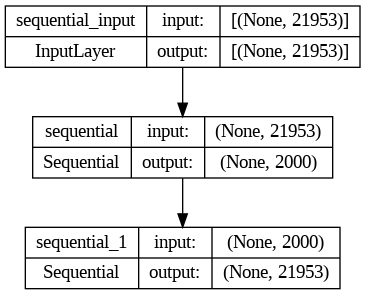
\includegraphics[width=.65\columnwidth]{./images/model.png}
        \captionof{figure}{Architecture of the autoencoder model.}
        \label{fig:architecture}
    }

    \vspace{1em}

    % results.tex
% Author: Tony Kabilan Okeke
% Date: 2023-03-23

\begin{figure*}[ht]
    \centering
    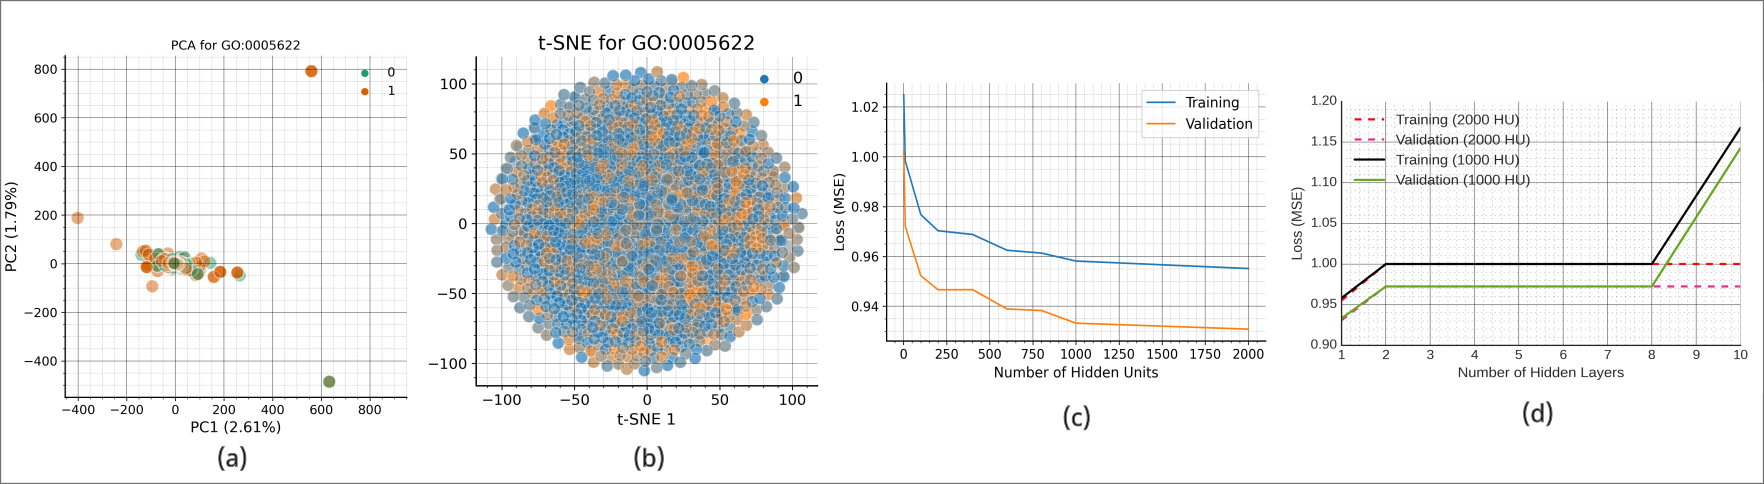
\includegraphics[width=\textwidth]{./images/results.png}
    \captionof{figure}{
        Results from evaluating the autoencoder.
        a) Scatter plot showing first 2 principal components of the data. Explained
        variances shown in axis labels.
        b) Scatter plot showing first 2 t-SNE components of the data.
        c) Autoencoder loss on the validation set with varied number of neurons.
        d) Autoencoder loss on the validation set with varied number of hidden layers.
    }
    \label{fig:results}
\end{figure*}

\section{Results}

First, we performed principal component analysis (PCA) on the logFC values to visualize
the data in a lower-dimensional space. The first two principal components explained
$2.61\%$ and $1.79\%$ of the total variance, respectively. Figure \ref{fig:results}a shows
the scatter plot of the first two principal components. The points are colored by whether
the GO0005622 (the most common GO term) term is enriched or not. No clear separation
between the two classes is observed.

\vspace{0.2cm}

We then visualized the data using t-distributed stochastic neighbor embedding (t-SNE).
Figure \ref{fig:results}b shows the scatter plot of the first two t-SNE components. The
points are colored by whether the GO0005622 term is enriched or not. Again, no clear
separation between the two classes is observed.

\vspace{0.2cm}

Next, we needed to determine the optimal number of neurons and hidden layers for the
autoencoder. To identify the optimal number of neurons, we trained the autoencoder with
varying numbers of neurons in a single hidden layer; we evaluated the model's performance
using the loss on the validation set. We tested the following numbers of neurons: 1, 10,
100, 200, 400, 600, 800, 1000, and 2000. Figure \ref{fig:results}c shows the loss on the
training and validation sets for each number of neurons. The loss on the validation set
decreased as the number of neurons increased, and plateaus at around 2000 neurons.

\vspace{0.2cm}

To identify the optimal number of hidden layers, we trained the autoencoder with varying
numbers of hidden layers. The total number of neurons in the network was first fixed at
2000 (the optimal number of neurons from the previous experiment), and subsequently at
1000. The neurons were distributed so each hidden layer had half the number of neurons
of the previous layer. We tested the following numbers of hidden layers: 1, 2, 3, 4, 5, 6,
7, 8, 9, and 10. Figure \ref{fig:results}d shows the loss on the training and validation
sets for each number of hidden layers. The loss on the validation set increased as the
number of hidden layers increased, with the lowest loss observed at 1 hidden layer.

\vspace{0.2cm}

Finally, we trained the autoencoder with the optimal number of neurons and hidden layers
(2000 neurons in a single hidden layer) over 50 epochs. The performance of the final model
was evaluated using 4-fold cross-validation. The average cross-validation loss was
$0.9632$.

    \vspace{1em}

    % discussion.tex
% Author: Tony Kabilan Okeke
% Date: 2023-03-23

\section{Discussion}

Our results provide insights into the use of autoencoders for unsupervised feature
learning from gene expression data. The performance of the autoencoder was evaluated
based on its ability to reconstruct the input data, and we believe that this is model
captures the underlying structure of the data well. However, we acknowledge some
limitations of our study. One major limitation was the memory constraints we faced
during training, which limited our ability to use all 48978 genes. In addition, we were
only able to evaluate a limited number of hyperparameters due to computational
limitations. Future studies could explore more advanced architectures such as sparse and
variational autoencoders to improve the performance of the model. Despite these
limitations, our study provides a foundation for future work in this area.
We plan to explore the use of the latent space of the autoencoder to perform feature
extraction for a classifier to predict the enrichment of Gene Ontology terms.

\vspace{0.2cm}

In summary, our work highlights the potential of autoencoders for unsupervised feature
learning from gene expression data, and provides a starting point for future studies to
explore more advanced architectures and evaluate the performance of the model on
predicting biological annotations. However, we acknowledge the limitations of our study
and the need for further research to address these limitations and advance the field.

    \vspace{1em}

    \bibliographystyle{ieeetr}
    \bibliography{includes/references}

    \balance
\end{multicols*}

\end{document}
